\documentclass[12pt,letter]{article}
\usepackage{tikz-qtree}

\usepackage[margin=1.0in]{geometry}

\begin{document}
\noindent\textsc{\large CS 314 Exam Review --- Get Grandparent}

\vspace{6pt}
\noindent\textbf{Binary Trees}

\vspace{2pt}
\noindent Write an instance method for a BinarySearchTree which, given an element
returns that element's grandparent in the tree. If the given element is not
in the tree, return \texttt{null}. If the element does not have a grandparent 
(i.e. the element is not deep enough), return the root element.

\vspace{4pt}
\noindent Complete the following method.
\begin{verbatim}
  // Returns the grandparent of 'data'
  // pre: data != null
  // post: This tree shall not be altered by this operation
  public E getGrandparent(E data){
\end{verbatim}

\vspace{4pt}

\noindent Here are some sample calls to \texttt{getGrandparent}: \newline

\tikzset{every tree node/.style={minimum width=2em,draw,circle},
         blank/.style={draw=none},
         edge from parent/.style=
         {draw,edge from parent path={(\tikzparentnode) -- (\tikzchildnode)}},
         level distance=1.5cm}
\texttt{b1 = }
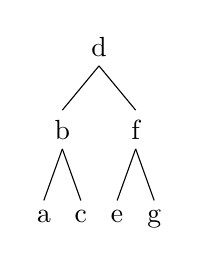
\begin{tikzpicture}
\Tree
[.d     
    [.b
      [.a
      ]
      [.c
      ]
    ]
    [.f
	  [.e
	  ]
	  [.g
	  ]
    ]
]
\end{tikzpicture}
\quad \texttt{b2 = }
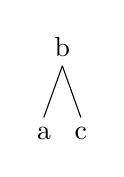
\begin{tikzpicture}
\Tree
[.b
  [.a
  ]
  [.c
  ]
]
\end{tikzpicture}
\quad\texttt{b3 = }
\begin{tikzpicture}
\Tree
[.y
  [.x
    [.w
	  [.v
	  ]
    \edge[blank]; \node[blank]{};
    ]
    \edge[blank]; \node[blank]{};
  ]
  [.z
  ]
]
\end{tikzpicture}
\newline

\begin{center}
\begin{tabbing}
\texttt{b1.getGrandparent('a') $\rightarrow$ 'd'} \quad 
\quad \quad \= \texttt{b1.getGrandparent('g') $\rightarrow$ 'd'} \\

\texttt{b2.getGrandparent('b') $\rightarrow$ 'b'} \> \texttt{b2.getGrandparent('c') $\rightarrow$ 'b'} \\
\texttt{b3.getGrandparent('a') $\rightarrow$ \texttt{null}} \> \texttt{b3.getGrandparent('v') $\rightarrow$ 'x'}
\end{tabbing}
\end{center}

\vspace{4pt}
\noindent You may use the following BinaryTree implementation

\begin{verbatim}
  public class BinarySearchTree<E extends Comparable<? super E>>{
    BSTNode<E> root;
    int size;

    //Nested node class
    private static class BSTNode<E>{
      BNode<E> left, right;
      E data;
    }
  }
\end{verbatim}

\noindent \textbf{Do not create any new data structures or use any other Java classes or methods.}

\clearpage
\begin{verbatim}
  // Returns the grandparent of 'data'
  // pre: data != null
  // post: This tree shall not be altered by this operation
  public E getGrandparent(E data){
\end{verbatim}
\end{document}
